\chapter{Conclusions} \label{chp:conclusion}
The ARC Stellar Mass Function plot at Figure \ref{fig:ARC_SMF} can give indicative information for order of magnitude since there are too little points for fitting a Schechter profile. For comparison, in Figure \ref{fig:SMF_Surv} the resulting Stellar Mass Function and its evolution for galaxies of the 3D-HST\cite{3DHST2012}\cite{3DHST2016} and COSMOS2015\cite{COSMOS152016} surveys are shown on the left panel\cite{Leja2020} and the local Universe SMF for the galaxies of the GAMA\cite{GAMA2009} survey are shown on the right panel\cite{Driver2022}, separately according to morphological type and in aggregate. GAMA is one of the most complete surveys with low median redshift, and the combined 3D-HST and COSMOS2015 surveys provide a very high completeness up to redshift $z=6$. \\
For the Local Universe, the NVSS-corrected ARC sample indicates a $\Phi$ of $\sim 10^{-4}$ galaxies per Mpc$^3$ for galaxy stellar mass of $\sim 10^{11} \,M_\odot$, which compared to the morphological SMF of the local Universe in Figure \ref{fig:SMF_Surv} is $\sim 1 $ dex lower than the local elliptical galaxies and $\sim 1$ to $2$ dex lower than all the local galaxies of the GAMA survey. It is an indication that in the local Universe gas rich radiogalaxies with stellar masses $> 10^{11}\,M_\odot$ are not as common as normal or elliptical galaxies, although at lower stellar masses ($\sim 10^{10.5}\, M)_\odot$ the Stellar Mass function is higher and could be percieved as an increase consistent with studies\cite{Tomczak2014} that support a rapid buildup for the lower mass quiescent sequence, potentially linking them to red quasars. This estimate is crude, since no exact values are compared, the literature results are not corrected to a Chabrier IMF to match the treatment of the ARC data, and it is not examined whether these studies are mass complete in the Chabrier IMF regime.\\
For the redshifts of $0.3<z<1.0$ the NVSS-corrected ARC sample indicates a $\Phi$ of $\sim 10^{-9}$ galaxies per Mpc$^3$ for galaxy stellar mass of $\sim 10^{11.5} \,M_\odot$, which, compared to the SMF of according redshift in the left panel of Figure \ref{fig:SMF_Surv}, is roughly $\sim 5$ dex lower. Similarly, for the redshift range of $1.0<z<2.5$, the the NVSS-corrected ARC sample SMF seems to be roughly $\sim 5$ dex lower, hinting that in higher redshift ARC-like radiogalaxies are even less common. \\
In Figure \ref{fig:ARC_SMF}, the disparity between the ARC galaxy density at different redshifts might be interpreted such that galaxies that evolve to be molecular gas-rich quasars (ARC-like) undergo this stage of evolution in the last $\sim 4$ Gyrs ($z<0.3$) of the Universe. Although, it is of central importance to highlight that the homogeneous (for every bin) NVSS completeness correction preformed in Section \ref{subsec:Res/ComplCorr} is a vast simplification, and more rigorous treatment is due that ought to take into account the impact of cosmic variance and integrate K-correction\cite{Kcorr2002}. \\
\begin{figure}[htbp]
   \subcaptionbox{3D-HST and COSMOS-2015 SMF evolution}{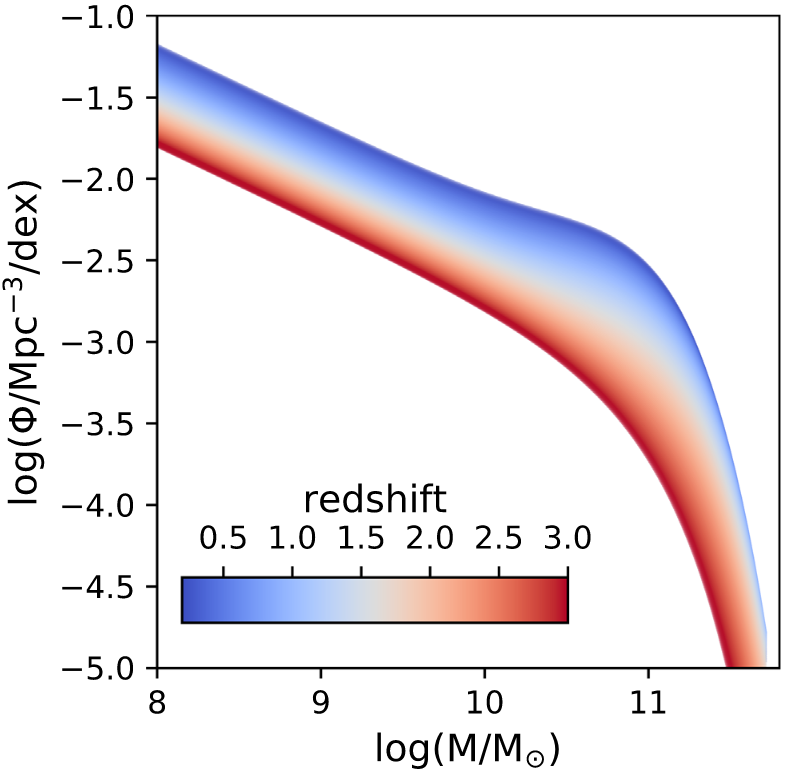
\includegraphics[width=0.4\linewidth]{figures/LejaSMF.png}}
    \subcaptionbox{GAMA Morphological SMF for local Universe}{ 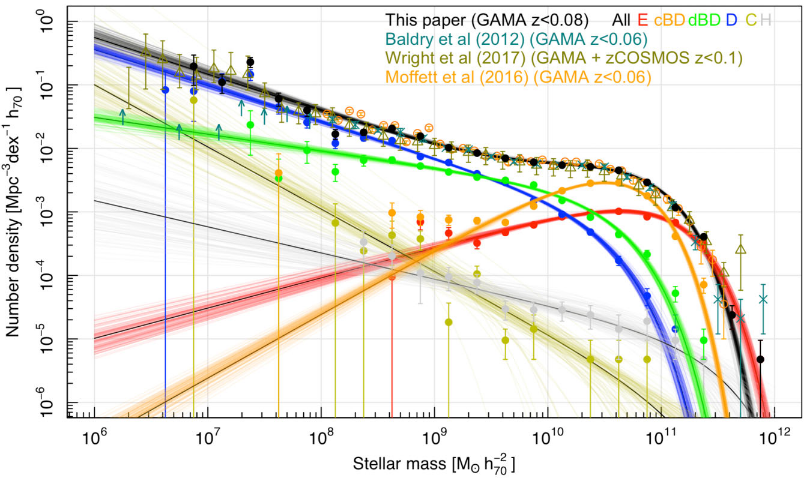
\includegraphics[width=0.59\linewidth]{figures/DriverSMF.png}}
    \caption{Comparison of Stellar Mass Function for different surveys. Figure lifted from Leja et al. (2020)\cite{Leja2020}. Figure lifted from Driver et al. (2022)\cite{Driver2022} }
    \label{fig:SMF_Surv}
\end{figure}
A case can also be made for the redshift bins since they include a wide interval of cosmic time, $\sim$ 3 or 4 Gyrs each, where many (not independent) stages of evolution are included.  \\ \\
In Figure \ref{fig:Gas-to-StarMassEvol} the molecular hydrogen gas mass-to-stellar mass ratio is plotted. This relation between gas and stars reveals the connection of star forming activity to
their immediate fuel. The molecular gas mass is estimated by Audibert et al. (2022)\cite{Audibert2022} from the CO spectroscopy. As shown in Figure \ref{fig:Gas-to-StarMassEvol}, the molecular gass mass-to-stellar mass ratio for the majority of the local ARC galaxies is weel bellow the relation of the CO-based molecular gas mass to stellar
mass ratio at the main-sequence from the work of Genzel et al.(2015)\cite{Genzel2015}, confirming that most ARC-like radiogalaxies in the local universe have already formed the majority of their stellar mass. Although in higher redshifts (i.e. $z>1.0$, corresponding to 8 or more Gyrs ago) they seem to be a lot closer to the main sequence hinting that they might be closer to their peak of star formation.\\

%%%%% Devies 2028 DEVILS 
%However, by design these surveys have targeted only the relatively local Universe (z < 0.3) % EXAMPLE Sloan Digital Sky Survey(SDSS, e.g. Abazajian et al. 2009), the Two Degree Field GalaxyRedshift Survey (2dFGRS
%While they provide a wealth ofinformation about galaxies at the current epoch, they cannot mea-sure the astrophysical processes that led to their formation. It is notthe processes occurring today that shaped the z ∼ 0 Universe butthe factors that drove galaxy evolution and structure formation overthe preceding contrary10 billion years.
%Very Large Telescope (VLT) VIsible Multi-Object Spectrograph (VIMOS) Deep Survey (VVDS, LeF‘evre et al. 2013), and VIMOS Ultra-Deep Survey (VUDS, LeF‘evre et al. 2015) have explored earlier epochs (z > 1)
%However, it is the relatively un-dersampled epoch at intermediate redshifts (0.3 < z < 1.0), whereboth galaxies and their host haloes undergo significant coeval evolu-tion, specifically in terms of the environmental effects on galaxies.At this epoch, many of the z ∼ 0 environmental trends observedin surveys such as GAMA and SDSS were shaped (e.g. Darvishet al. 2016). It is here that roughly half of all stars were formed(Madau & Dickinson 2014; Driver et al. 2018); galaxies underwentsignificant mass, size, morphology, and angular momentum evolu-tion (e.g. Lotz et al. 2011; van der Wel et al. 2012; Codis, Pichon &Pogosyan 2015; Lange et al. 2015); and our current cold dark mattermodel CDM predicts a strong and testable evolution of the halomass function (e.g. Murray, Power & Robotham 2013; Elahi et al.2018). Surprisingly, this key epoch in the formation of the funda-mental relationships we observe today has been left comparativelyunexplored

\section{Improvements \textit{\&} Future Work}

The projection of the modelled SED to model photometry is described in Section \ref{sec:filters}, and includes the use of filter curves, which are excluded from the present work. A careful selection of every filter curve corresponding to the observational data will contribute to a more rigorous treatment of SED fitting.\\
As highlighted in Section \ref{sec:SFH}, modeling the Star Formation History with a functional form is prone to inaccurate modelling of a galaxy's SED. As shown in Table \ref{tab:ParamSpace}, two composite stellar population models of delayed exponential decay SFH are used, differing in age, so that a more complex SFH function could be modeled, although there is vast room for improvement. A basis of nonparametric\cite{Iyer2019} Star Formation Histories can be built by training with a well motivated selection of SFH families\cite{Iyer2017} or generate stochastic SFHs. This can result to a more complete formulation of SFH and the use of one well-informed composite stellar population component which means a robust estimation\cite{Lower2020} of not only Star Formation Rate, but also mass-weighted ages.\\
As discussed in Section \ref{sec:blazar}, the implemented SED models in the present work lack a blazar component, which is crucial for improvement of the routine since many of the ARC galaxies are radio loud balzars and including the appropriate modelling can expand the current sample of reliably fitted galaxies. Blazar SED components can be fitted with robust modeling\cite{Petropoulou2015}, and is a central priority for the amelioration of the present code. \\
Imposing priors of the separate AGN torus parametres can lead to a more careful SED fitting, especially if blazars are going to be fitted, in which case physical quantities such as inclination can be coupled with the blazar emission component (as demonstrated in Figure \ref{fig:AGNUni}).\\
Imposition of a prior on the accretion disk emission upper limit from HST observations of the central region of the resolved sources, which is a proxy of the AGN fraction, makes the SED modelling astrophysically sounder. Although it has been tested, a more thorough selection of upper limits is due and will be implemented in an improved version of the code, as mentioned in Section \ref{sec:priors}.\\
In dust attenuation equation \ref{eq:dustatten} the 0.4 attenuation for local universe is adopted, while 0.93 for $z \sim 1$ is proposed by Puglisi et al. (2016)\cite{Pugli2016}, although Narayanan et al. (2023)\cite{Narayanan2023} and Lower et al. (2023)\cite{Lower2023} remark that the choice of attenuation law contributes to the stellar component shape significantly less than the assumed Star Formation History.\\
Advanced methods for Stellar Population Synthesis could be an update for the future, such as  Differentiable Stellar Population Synthesis(DSPS)\cite{Hearin2023} or use of emulators\cite{Kwon2023} along with nonparametric prescriptions for the SFH (already discussed).\\
As demonstrated in Section \ref{sec:Likeli}, in the formulation of the Bayesian likelihood the covariance matrix can be specified as a sum of weighted kernels for noise models, which is useful if spectroscopic data form galaxies should be used. Some of the ARC galaxies have IR spectral data from Spitzer/IRS, which have not been used for the analysis of the present thesis. Careful noise modeling ought to be invoked when spectrograms are included.\\ \\
Methodical modelling of SFH can lead to the estimation of Star Formation Rate at any given time, and better assessment of the radiogalaxy evolution in the last $\sim$ 11 Gyrs. 
The Stellar Mass Function could be better corrected for completeness, and stellar masses can be inferred for a larger sample when including a blazar component. The stellar mass and dust mass will be inferred more robustly with one composite stellar population and thorough SFH modelling. 
Scaling relations such as molecular gas mass-to-stellar mass ratio evolution and inferred dust mass-to-stellar mass ratio can be produced and studied with representative uncertainties. 
In conclusion, improvement on the fitting method, in particular
\begin{itemize}
    \item the Star Formation History modelling and computational implementation
    \item correct filter integration and application
    \item extension of the model to include a rigorous blazar component fit
\end{itemize}
can lead to more robust results without resorting to the request of high resolution spectroscopy as well as including more galaxies to the studied sample.\\
A more careful treatment of the post processing methods, such as the completeness correction, inclusion of cosmic variance and Bayesian inference integrated K-correction can vastly improve the conclusiveness of the results and the comparison with literature.


